\documentclass[convert={density=300,outext=.png}]{standalone}
\usepackage{tikz}

\begin{document}
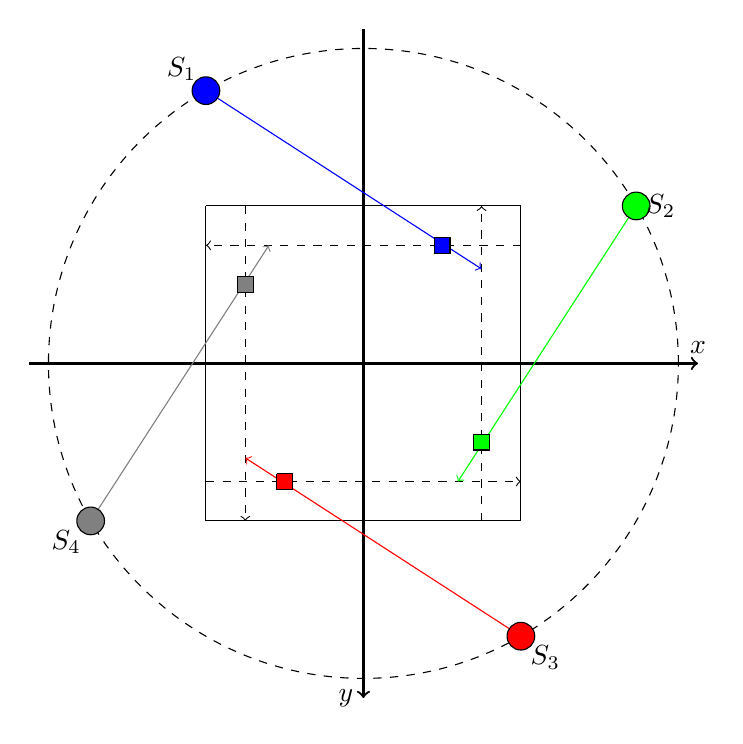
\begin{tikzpicture}[axis/.style={thick,->}]
    \draw[axis] (0, 4.25, 0) -- (0, -4.25, 0) node [left] {$y$};
    \draw[axis] (-4.25, 0, 0) -- (4.25, 0, 0) node [above] {$x$};

    % Volumen
    \draw (-2, 2, 0) -- (2, 2, 0) -- (2, -2, 0) -- (-2, -2, 0) -- (-2, 2, 0);

    % Pfeile im Volumen
    \draw[dashed,->] (-1.5, 2, 0) -- (-1.5, -2, 0);
    \draw[dashed,->] (2, 1.5, 0) -- (-2, 1.5, 0);
    \draw[dashed,->] (1.5, -2, 0) -- (1.5, 2, 0);
    \draw[dashed,->] (-2, -1.5, 0) -- (2, -1.5, 0);

    % Kreis
    \draw[dashed] (0, 0, 0) circle [radius=4];

    % Quellpfeile
    \draw[color=blue,->] (-2, 3.46410) -- (1.5, 1.2);
    \draw[color=green,->] (3.46410, 2) -- (1.2, -1.5);
    \draw[color=red,->] (2, -3.46410) -- (-1.5, -1.2);
    \draw[color=gray,->] (-3.46410, -2) -- (-1.2, 1.5);

    % Quellpositionen
    \draw[fill=blue] (-2, 3.46410) circle (5pt) node [above left] {$S_1$};
    \draw[fill=green] (3.46410, 2) circle (5pt) node [right] {$S_2$};
    \draw[fill=red] (2, -3.46410) circle (5pt) node [below right] {$S_3$};
    \draw[fill=gray] (-3.46410, -2) circle (5pt) node [below left] {$S_4$};

    % Voxel
    \draw[fill=blue] (0.9, 1.6) -- (1.1, 1.6) -- (1.1, 1.4) -- (0.9, 1.4) -- (0.9, 1.6);
    \draw[fill=green] (1.4, -0.9) -- (1.6, -0.9) -- (1.6, -1.1) -- (1.4, -1.1) -- (1.4, -0.9);
    \draw[fill=red] (-1.1, -1.4) -- (-0.9, -1.4) -- (-0.9, -1.6) -- (-1.1, -1.6) -- (-1.1, -1.4);
    \draw[fill=gray] (-1.6, 1.1) -- (-1.4, 1.1) -- (-1.4, 0.9) -- (-1.6, 0.9) -- (-1.6, 1.1);
\end{tikzpicture}
\end{document}
